\documentclass{article}
\usepackage{fancyhdr}
\usepackage{amsmath,amssymb}
\usepackage{geometry}
\usepackage{datetime}
\usepackage{enumerate}
\usepackage{graphicx}

%Insert page formatting here
\hoffset = -.5in
\voffset = -0.375in
\textwidth = 7in
\textheight = 8in
\headheight = 24pt

\pagestyle{fancy}

\rhead{Peter Olson\\Student ID: $441666$}
\lhead{Math 3200\\Homework 10}
\chead{\today}
\cfoot{}

%\addtolength{\headwidth}{\marginparsep}
%\addtolength{\headwidth}{\marginparwidth}

%\renewcommand{\labelitemi}{$\diamond$}
\renewcommand{\implies}{\rightarrow}
\newcommand{\widespace}{\qquad \qquad \;}
\newcommand{\tret}{\\ \hline}
\newcommand{\fh}{\tfrac{1}{2}}
\newcommand{\deriv}[2]{\frac{d #1}{d #2}}
\newcommand{\pderiv}[2]{\frac{\delta #1}{\delta #2}}
\newcommand{\vr}{\vec{r}}
\newcommand{\at}{\text{ at }}
\newcommand{\var}{\text{Var}}
\newcommand{\cov}{\text{Cov}}

\begin{document}

\section*{Exercise 10.20}

\begin{enumerate}[\quad(a)]
	\item Fit an LS straight line to these data. Plot the residuals against the speed.\\
	\begin{center}
		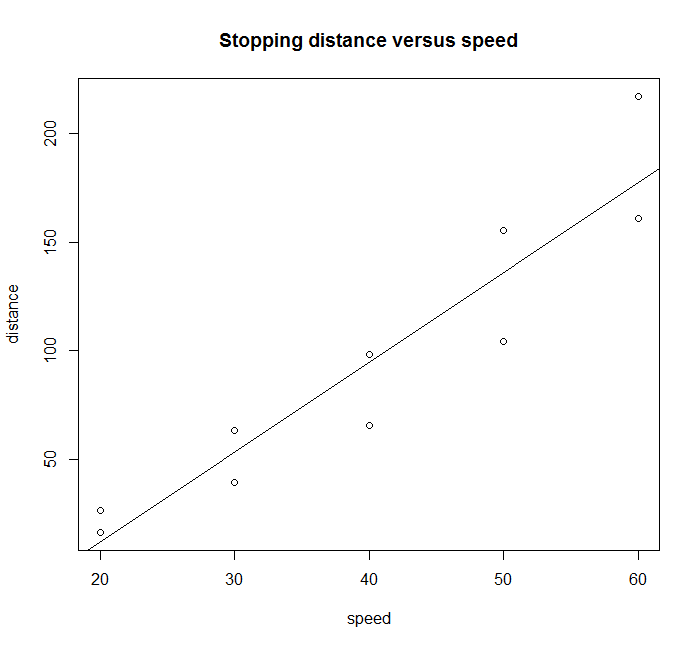
\includegraphics[width=3in]{Q51.png}$\qquad$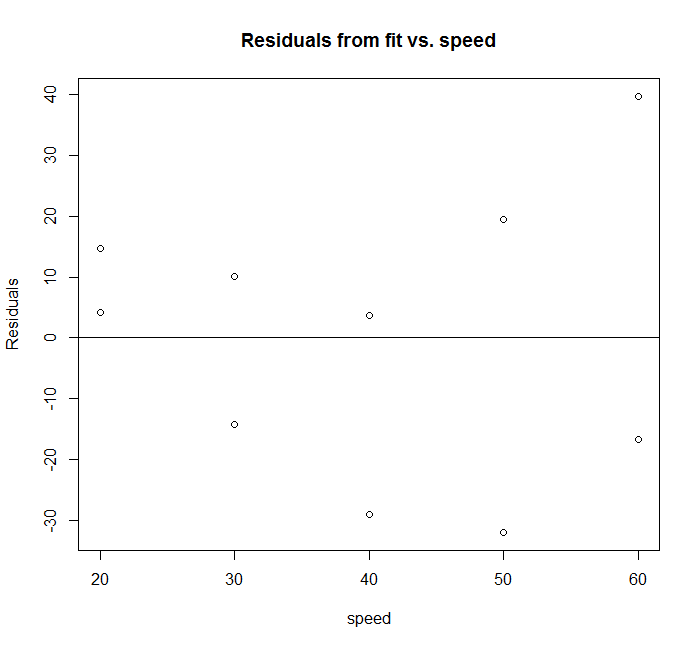
\includegraphics[width=3in]{Q52.png}
	\end{center}
	\item Commend on the goodness of the fit based on the overall F-statistic and the residual plot. Which two assumptions of the linear regression model seem to be violated?

	While the F-statistic is very high (\texttt{58.76821}), the data appears to violate assumption one, that ``the mean of $Y_i$ is a linear function of $x_i$'', based on the two curves that seem to appear in the residual graph.
	\item What transformation of stopping distance should be used to linearize the relationship with respect to speed?

	Given what I know about the relationship between kinetic energy and velocity, the stopping distance should be square-rooted to create a linear relationship with the speed.
	\newpage
	\item Make this linearizing transformation and check the goodness of the fit. What is the predicted stopping distance according to this model if the car is travelling at 40 mph?\\
	\begin{center}
		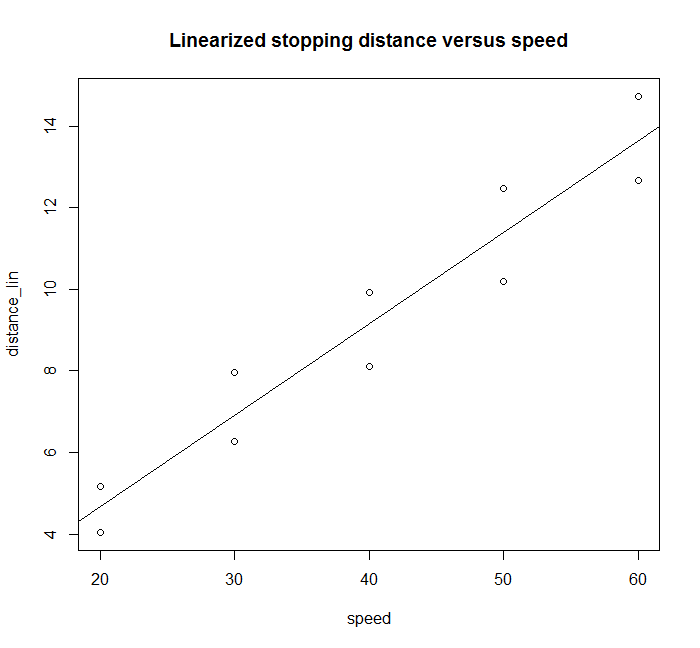
\includegraphics[width=3in]{Q53.png}$\qquad$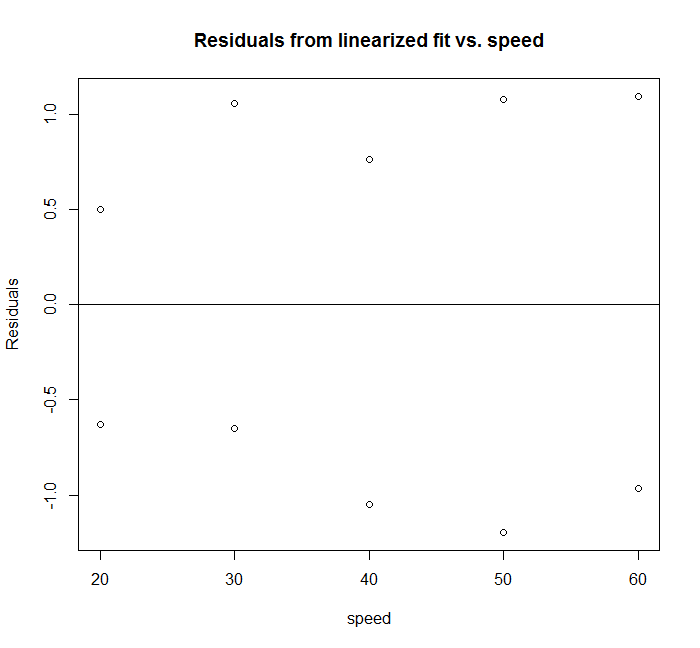
\includegraphics[width=3in]{Q54.png}
	\end{center}

	This linearized distribution has a better F-statistic, and an even lower p-value.

	Given how the data is taken using ten different cars, with different weights, internal components, and tires, even in potentially different road conditions, it seems foolish to use this data as the basis for any expectation on how long it should take some arbitrary car to stop. 

	However, the 95\% prediction interval for a car moving at 40 mph is $[93.1131, 96.3869]$ meters.
\end{enumerate}

\section*{R Output}
\begin{verbatim}
> # echo out F-statistic
> summary(fit)

Call:
lm(formula = distance ~ speed)

Residuals:
   Min     1Q Median     3Q    Max 
-32.00 -16.04   3.95  13.51  39.75 

Coefficients:
            Estimate Std. Error t value Pr(>|t|)    
(Intercept) -70.6500    22.8845  -3.087    0.015 *  
speed         4.1350     0.5394   7.666 5.93e-05 ***
---
Signif. codes:  0 ‘***’ 0.001 ‘**’ 0.01 ‘*’ 0.05 ‘.’ 0.1 ‘ ’ 1

Residual standard error: 24.12 on 8 degrees of freedom
Multiple R-squared:  0.8802,	Adjusted R-squared:  0.8652 
F-statistic: 58.77 on 1 and 8 DF,  p-value: 5.928e-05

> # echo out F-statistic
> summary(fit_lin)

Call:
lm(formula = distance_lin ~ speed)

Residuals:
     Min       1Q   Median       3Q      Max 
-1.19628 -0.88439 -0.06571  0.98377  1.09473 

Coefficients:
            Estimate Std. Error t value Pr(>|t|)    
(Intercept)  0.18048    0.98273   0.184    0.859    
speed        0.22437    0.02316   9.687 1.08e-05 ***
---
Signif. codes:  0 ‘***’ 0.001 ‘**’ 0.01 ‘*’ 0.05 ‘.’ 0.1 ‘ ’ 1

Residual standard error: 1.036 on 8 degrees of freedom
Multiple R-squared:  0.9214,	Adjusted R-squared:  0.9116 
F-statistic: 93.83 on 1 and 8 DF,  p-value: 1.076e-05


> # echo out prediction
> predict(fit, newspeed, level = 0.05, interval="predict")
    fit     lwr     upr
\end{verbatim}

\section*{R Code}
\begin{verbatim}
# Prepare data
speed <- c(
  20, 20, 
  30, 30, 
  40, 40, 
  50, 50, 
  60, 60
)

distance <- c(
  16.3, 26.7,
  39.2, 63.5,
  65.7, 98.4,
  104.1, 155.6,
  217.2, 160.8
)

# a

plot(speed, distance, main = "Stopping distance versus speed")

fit = lm(distance~speed)
abline(fit)

plot(speed, fit[['residuals']], ylab = "Residuals", main = "Residuals from fit vs. speed")
abline(0,0)

# b
# echo out F-statistic
summary(fit)

# c

distance_lin = sqrt(distance)

# d

plot(speed, distance_lin, main = "Linearized stopping distance versus speed")

fit_lin = lm(distance_lin~speed)
abline(fit_lin)

plot(speed, fit_lin[['residuals']], ylab = "Residuals", main = "Residuals from linearized fit vs. speed")
abline(0,0)

# echo out F-statistic
summary(fit_lin)

# create dataframe for prediction
newspeed <- data.frame(speed=40)
# echo out prediction
predict(fit, newspeed, level = 0.05, interval="predict")

\end{verbatim}

\end{document}